\documentclass[border=0.8ex,svgnames,tikz]{standalone}
\usepackage{amsmath,mathtools}
\usepackage{fontspec}
\setmainfont{Source Serif 4}
\setsansfont{Source Sans 3}
\setmonofont{Source Code Pro}
\usetikzlibrary{positioning,shapes.multipart}
\begin{document}
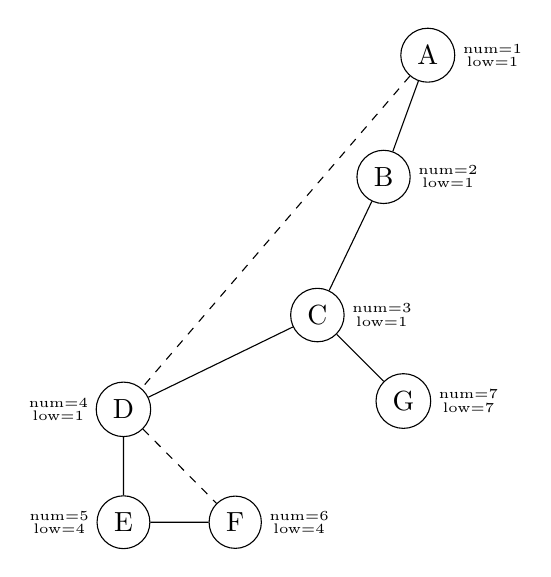
\begin{tikzpicture}
  \begin{scope}[every node/.style={draw,circle,minimum size=1.8em}]
    \coordinate(graph) at(0,0);
    \node[below=of graph] (graphA) {A};
    \node[below left=3em and 0.2em of graphA] (graphB) {B};
    \node[below left=3.6em and 1em of graphB] (graphC) {C};
    \node[below right=2.4em of graphC] (graphG) {G};
    \node[below left=2em and 5.6em of graphC] (graphD) {D};
    \node[below=2.1em of graphD] (graphE) {E};
    \node[right=2.1em of graphE] (graphF) {F};
  \end{scope}
  \begin{scope}[
    node distance=.5ex,
    every node/.style={
      font=\tiny,
      align=center,
      inner sep=0.1ex,
      rectangle split,
      rectangle split ignore empty parts,
    },
    ]
    \node[right=of graphA]{num=1 \nodepart{two}low=1};
    \node[right=of graphB]{num=2 \nodepart{two}low=1};
    \node[right=of graphC]{num=3 \nodepart{two}low=1};
    \node[right=of graphG]{num=7 \nodepart{two}low=7};
    \node[left=of graphD]{num=4 \nodepart{two}low=1};
    \node[left=of graphE]{num=5 \nodepart{two}low=4};
    \node[right=of graphF]{num=6 \nodepart{two}low=4};
  \end{scope}
  \begin{scope}[
    every path/.style={draw},
    backp/.append style={dashed},
    ]
    \path
    (graphA) -- (graphB) -- (graphC) -- (graphD) -- (graphE) -- (graphF)
    (graphC) -- (graphG);
    \path[backp] (graphA) -- (graphD) -- (graphF);
  \end{scope}
\end{tikzpicture}
\end{document}
